\chapter{Testování}
\label{chap:testovani}

%%%%%%%%%%%%%%%%%%%%%%%%%%%%%%%%%%%%%
%	LOD0 vs LOD1
%
obrázek scény A
\begin{figure}[here]
\begin{center}
$\begin{array}{ccc}
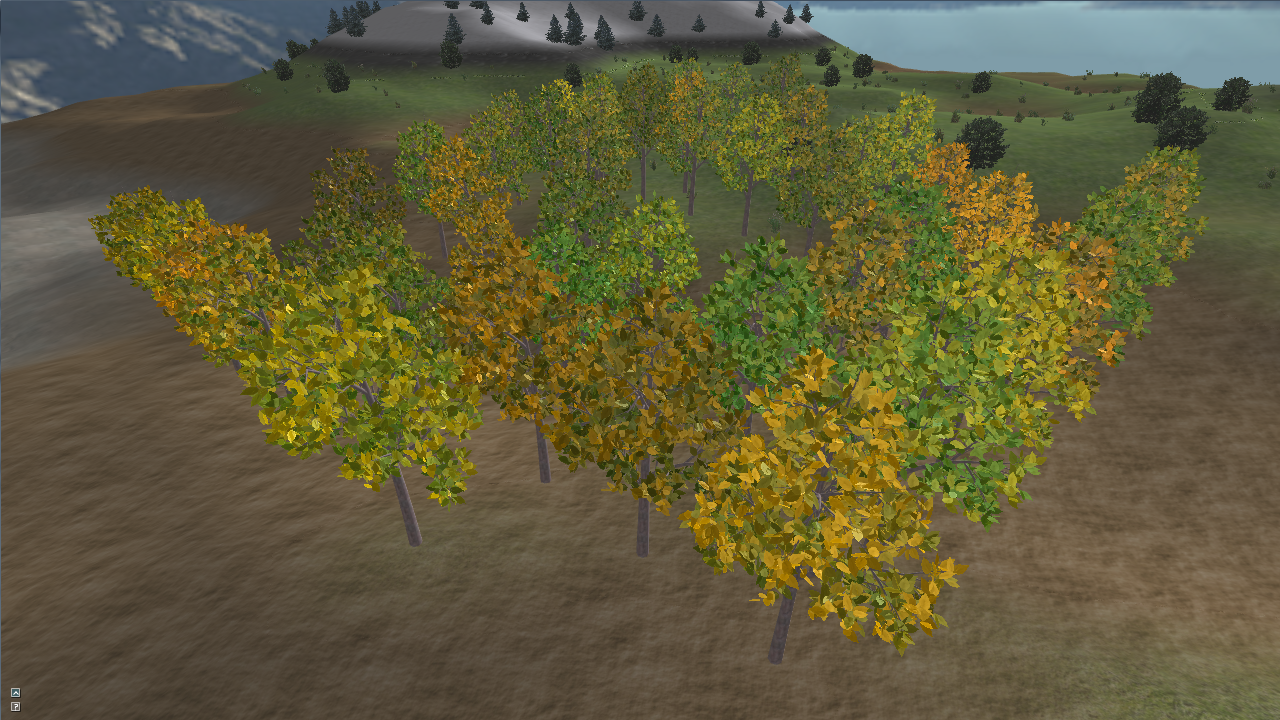
\includegraphics[width=0.3\textwidth]{./testing/LOD0only50.png}&
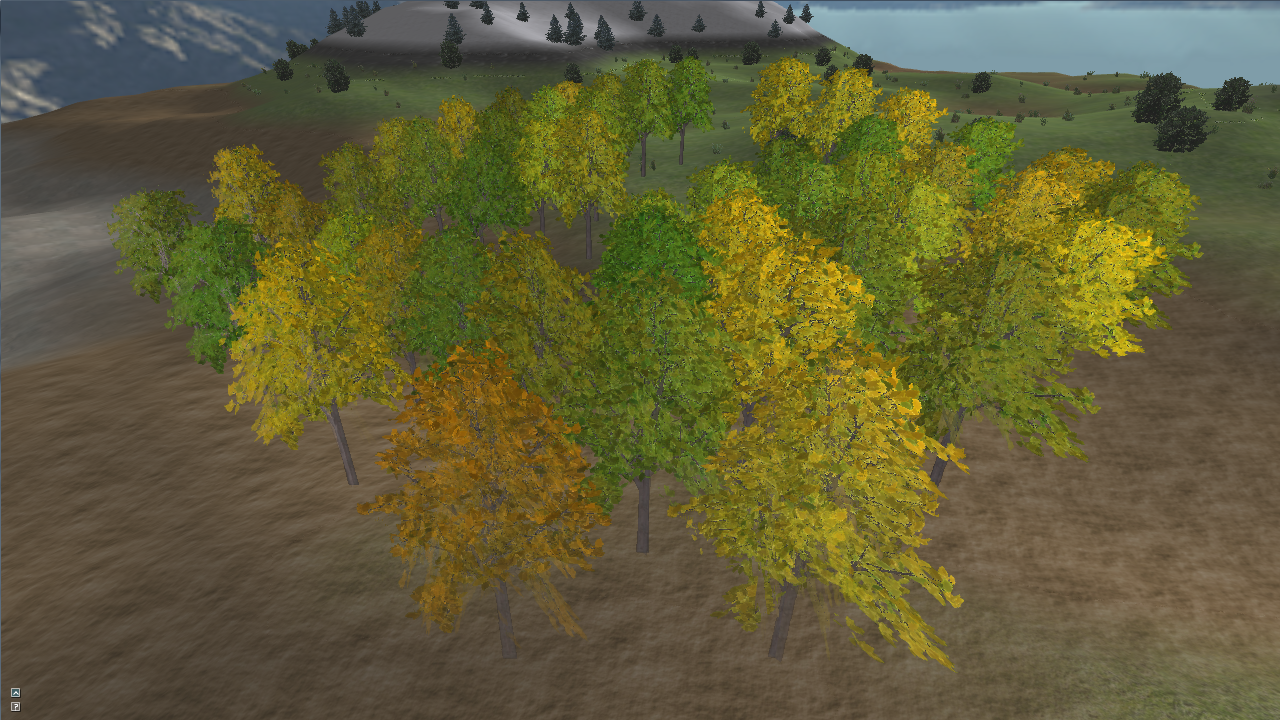
\includegraphics[width=0.3\textwidth]{./testing/LOD1only50.png}&
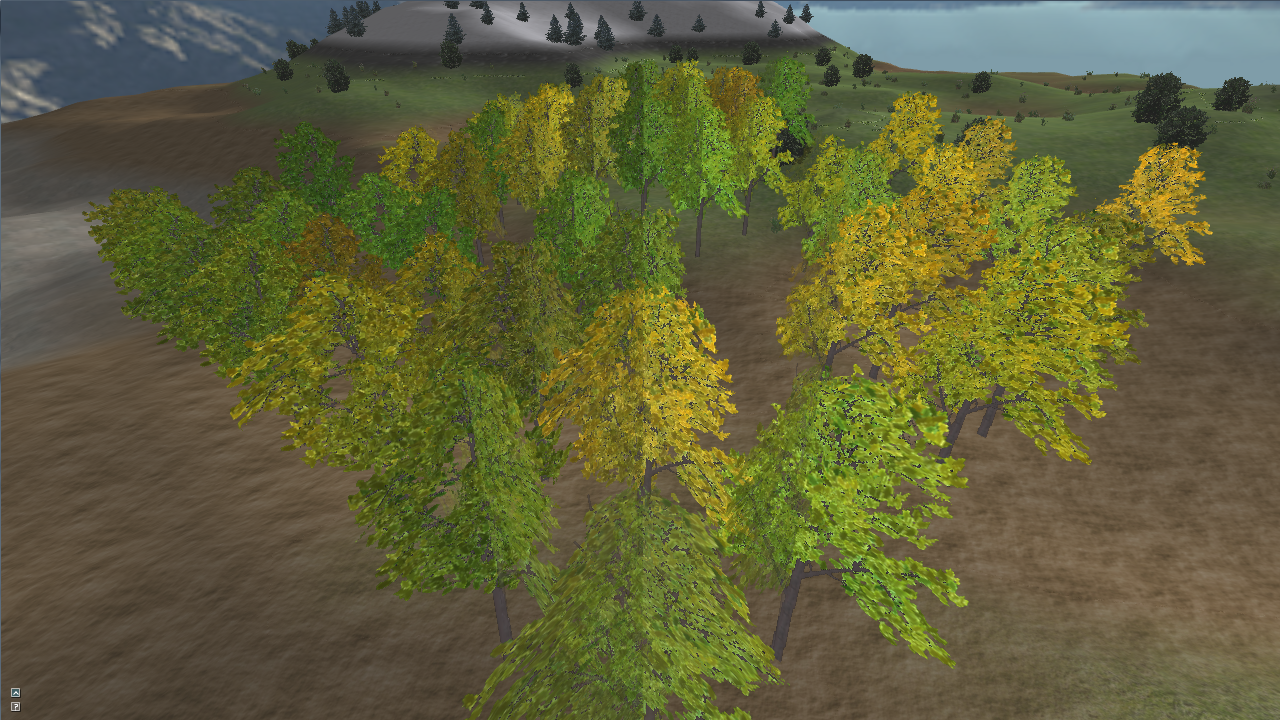
\includegraphics[width=0.3\textwidth]{./testing/LOD2only50.png}
\\
(a)&(b)&(c)
\end{array}$
\end{center}
\caption[Náhledy testovací scény]%
{Náhledy z testování, scéna SMALL FOREST s 50 instancemi, (a) LOD0,  (b) LOD1, (c) LOD2, 0\label{fig:testONLYsmal}
}
\end{figure}
obrázek scény B
\begin{figure}[here]
\begin{center}
$\begin{array}{ccc}
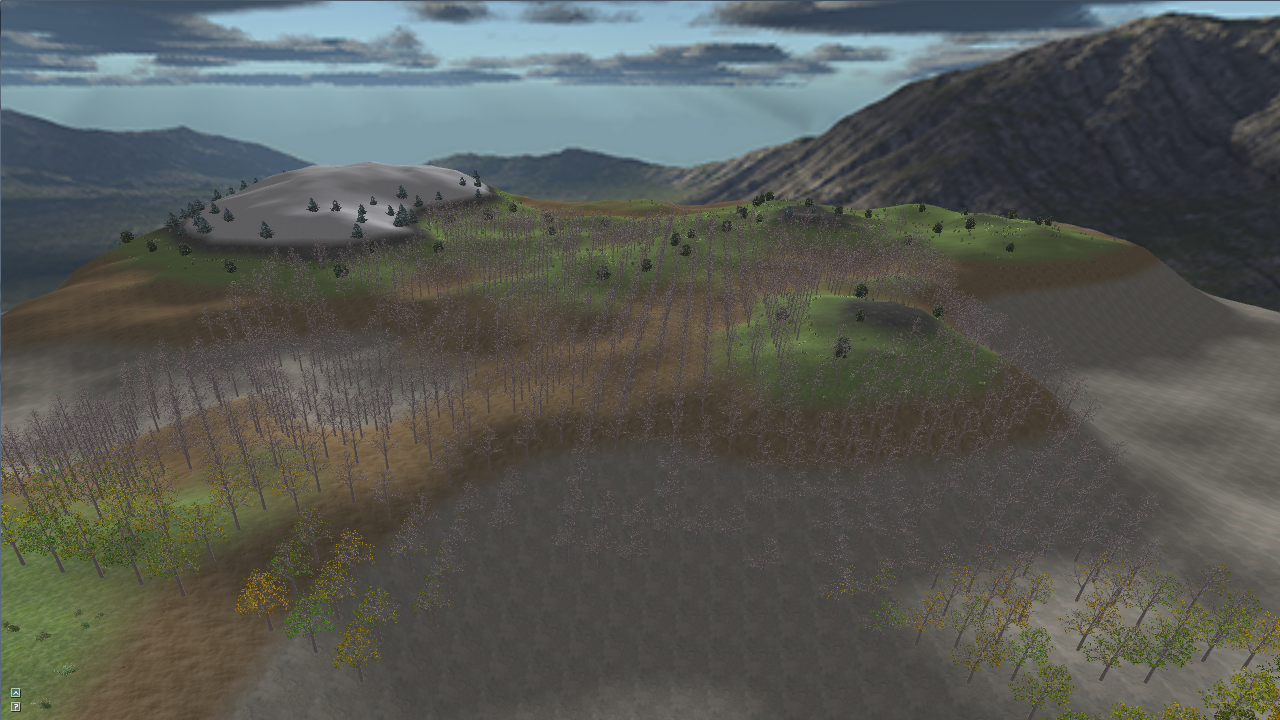
\includegraphics[width=0.3\textwidth]{./testing/LOD0only1000.png}&
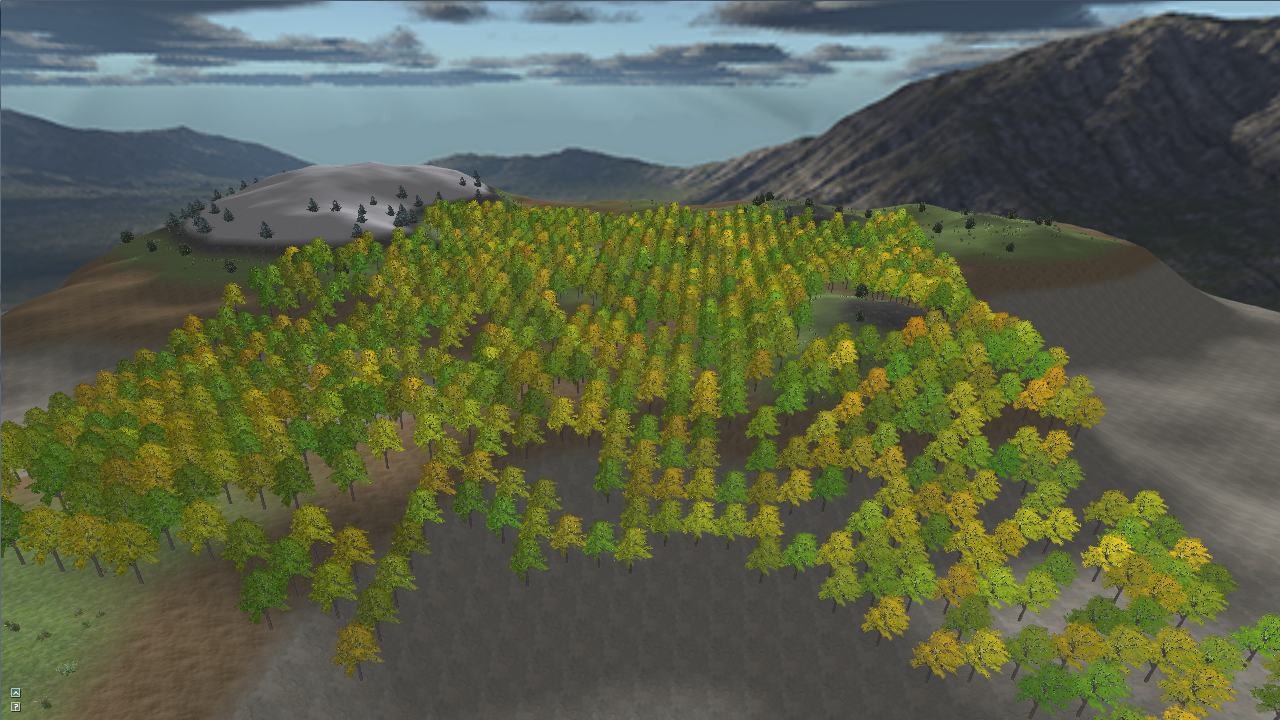
\includegraphics[width=0.3\textwidth]{./testing/LOD1only1000.png}&
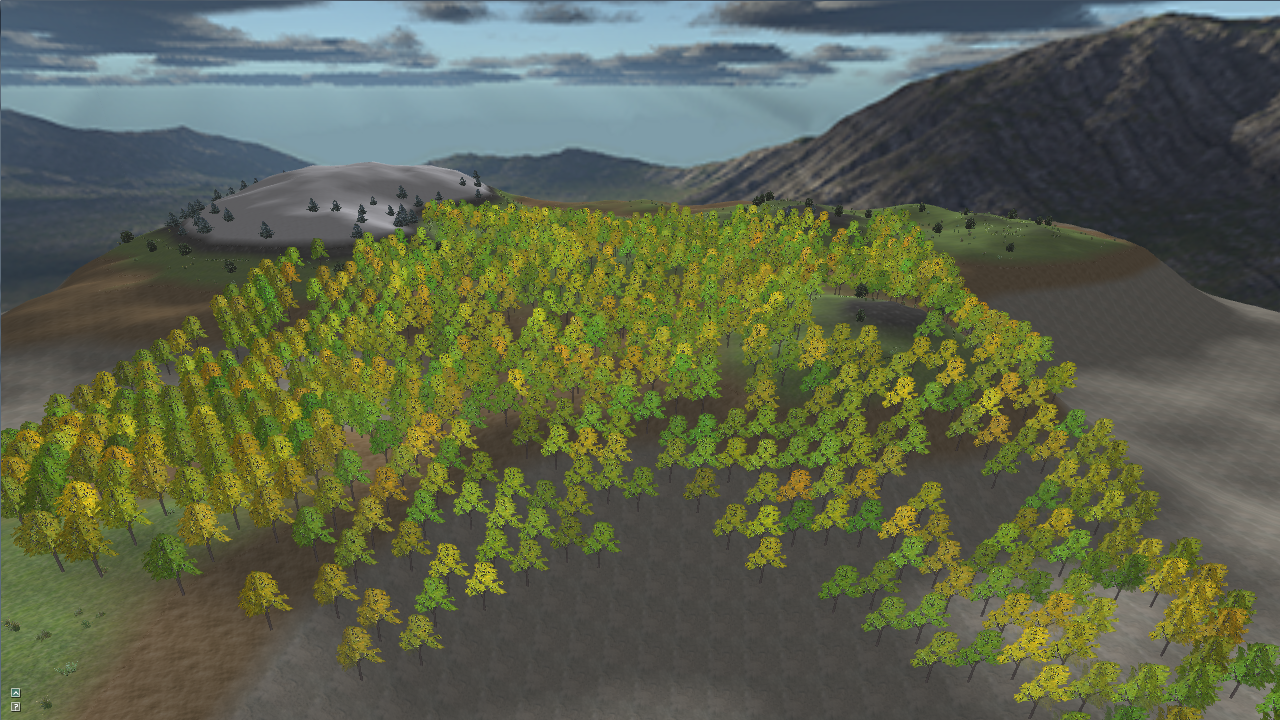
\includegraphics[width=0.3\textwidth]{./testing/LOD2only1000.png}
\\
(a)&(b)&(c)
\end{array}$
\end{center}
\caption[Náhledy testovací scény]%
{Náhledy z testování, scéna FOREST s 1000 instancemi , (a) LOD0,  (b) LOD1, (c) LOD2, 0\label{fig:testONLYl}
}
\end{figure}

porovnání kvality při pohledu z dálky

\begin{figure}[here]
\begin{tabular}{r l}
LOD0 & 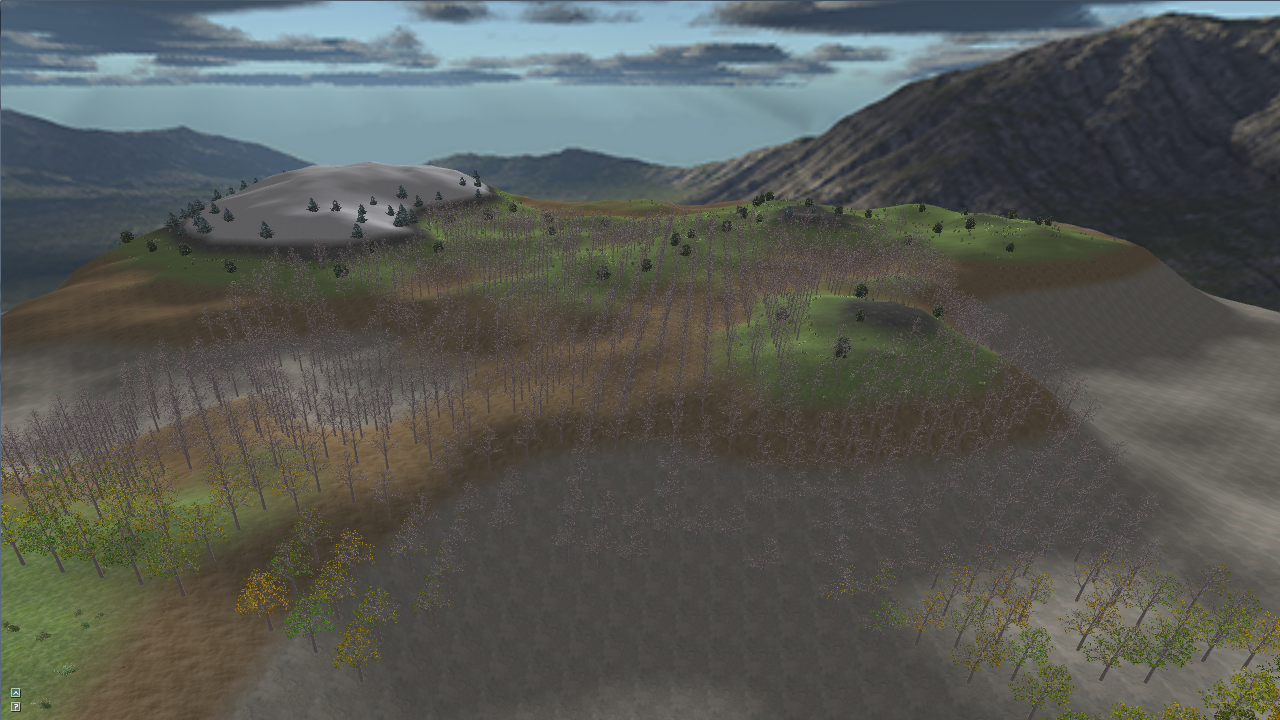
\includegraphics[width=0.9\textwidth]{./testing/LOD0only1000.png}\\
LOD1 & 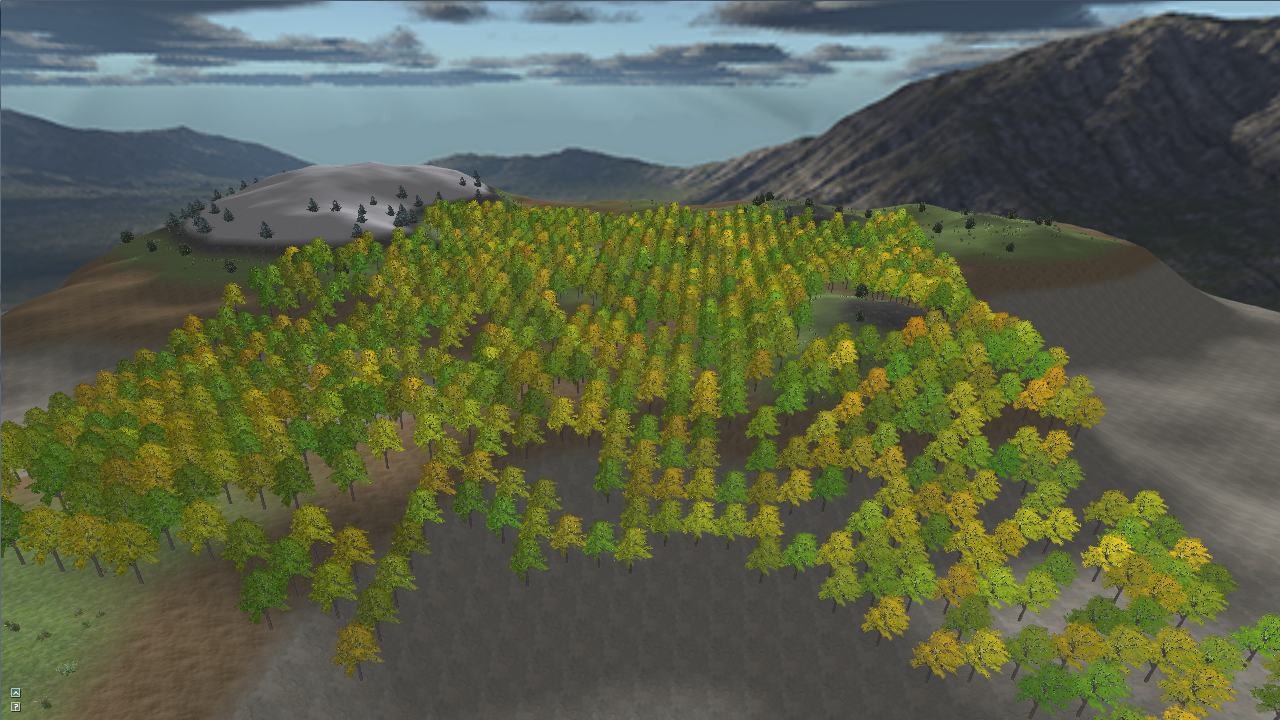
\includegraphics[width=0.9\textwidth]{./testing/LOD1only1000.png}\\
\end{tabular}
\caption[Náhledy testovací scény]%
{Náhledy z testování, scéna FOREST s 1000 instancemi, porovnání výsledné kvality \label{fig:testQuality}
}
\end{figure}



\begin{table}[here]
\centering
\begin{tabular}{|r | c | c | l |} 
\hline 
\#instancí & LOD0 (ms)& LOD1 (ms)& \\ [0.5ex] 
\hline
10	&	2,98	&	3,71	& 	\multirow{3}{*}{scéna A}\\
25	&	7,37		&	8,96	&	 \\
50	&	13,71	&	16,89	&	 \\
\hline
100	& 	20,25	&	6,54	&	\multirow{4}{*}{scéna B}\\
250	& 	48,15	&	15,59	&\\
500	& 	94,73 	& 	30,36	&\\
1000 & 	188,96 	& 	57,16	&\\
 [1ex] 
\hline 
\end{tabular}
\label{table:lod01-1MS}
\caption{Porovnání LOD0 a LOD1, bez multisamplingu}

\end{table}

\begin{table}[here]
\centering
\begin{tabular}{|r | c | c | l |} 
\hline 
\#instancí & LOD0 (ms)& LOD1 (ms)& \\ [0.5ex] 
\hline
10	&	3,72	&	4,26	& 	\multirow{3}{*}{scéna A}\\
25	&	8,32	&	9,48	&	 \\
50	&	15,94	&	16,5	&	 \\
\hline
100	& 	19,34	&	6,04	&	\multirow{4}{*}{scéna B}\\
250	& 	47,5		&	14,36	&\\
500	& 	94,2 	& 	28,58	&\\
1000 & 	188,3 	& 	55,87	&\\
 [1ex] 
\hline 
\end{tabular}
\label{table:lod01-4MS}
\caption{Porovnání LOD0 a LOD1, 4x multisampling}
\end{table}


%%%%%%%%%%%%%%%%%%%%%%%%%%%%%%%%%%%%%
%	Fragmenty vs čas, 1 strom různé vzdálenosti
%
\begin{table}[here]
\centering
\begin{tabular}{|r | c | c | c | c | c | c |} 

\hline 
& \multicolumn{3}{|c|}{LOD0}& \multicolumn{3}{|c|}{LOD1}\\
vzdálenost & \# fragmentů & fps & čas (ms) & \# fragmentů & fps & čas (ms)\\ [0.5ex] 
\hline
50		&6734		&1693,29	&0,59	&4226		&1391,3		&0,71875\\
40		&10537		&1538,84	&0,65	&7662		&1268,64	&0,78825\\
30		&18886		&1263,75	&0,79	&15379		&1183,22	&0,84515\\
20		&43139		&928,04		&1,08	&39297		&1018,22	&0,98211\\
10		&180614	&389,14		&2,57	&185531	&665,14		&1,50345\\
 [1ex] 
\hline 
\end{tabular}
\label{table:lod01-fragtime}
\caption{Závislost zobrazovacího času na počtu fragmentů}

\end{table}
nahledy
\begin{figure}[here]
\begin{center}
$\begin{array}{ccccc}
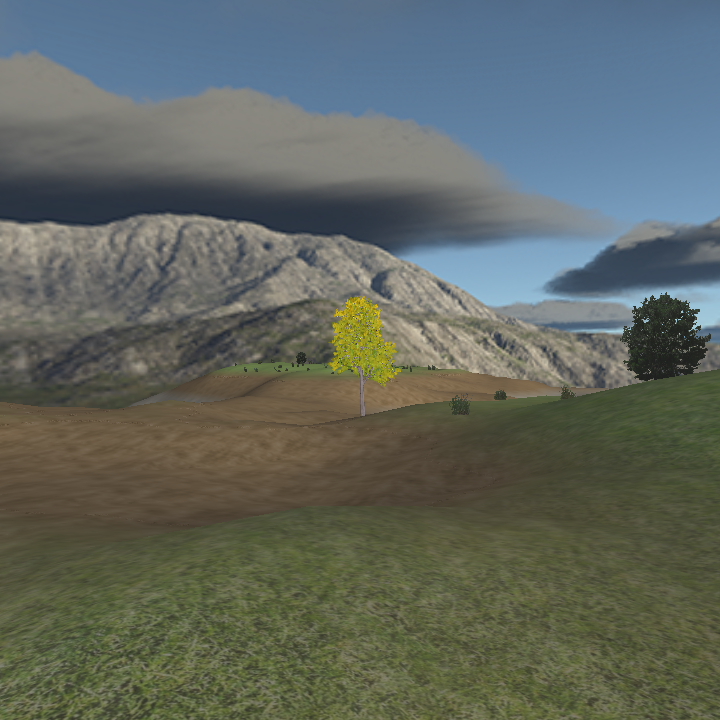
\includegraphics[width=0.17\textwidth]{./testing/LOD1-d50.png}&
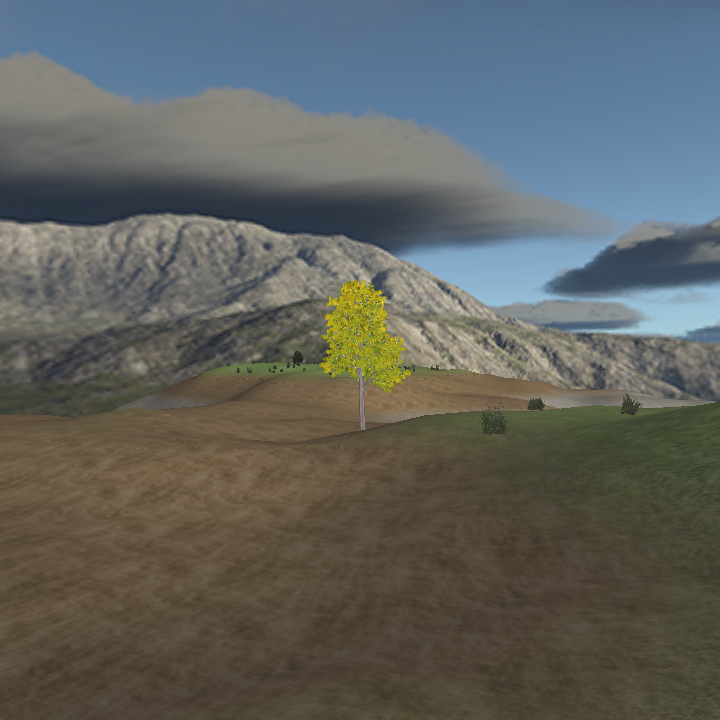
\includegraphics[width=0.17\textwidth]{./testing/LOD1-d40.png}&
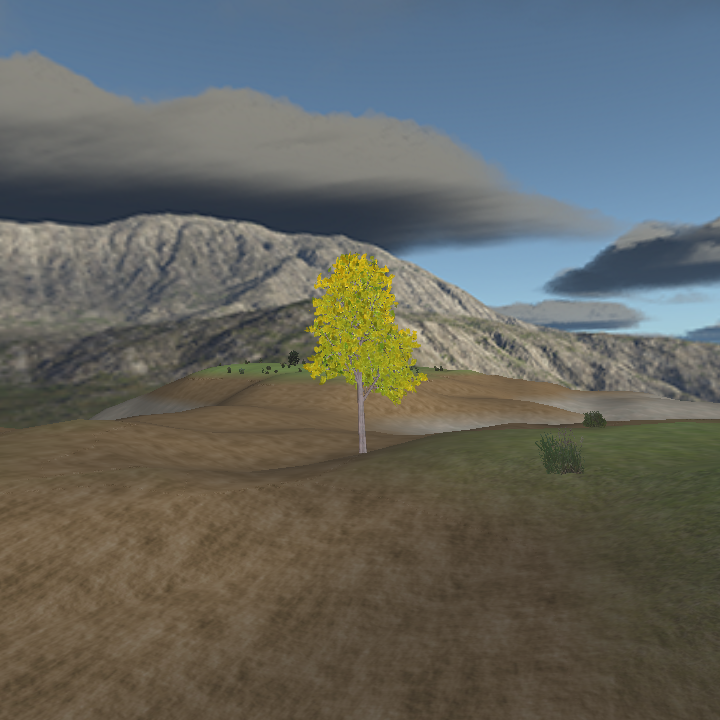
\includegraphics[width=0.17\textwidth]{./testing/LOD1-d30.png}&
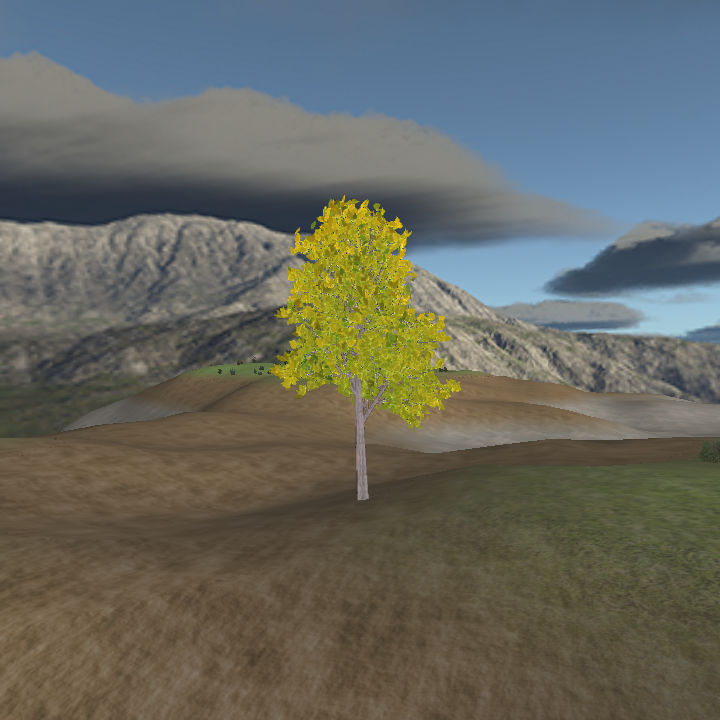
\includegraphics[width=0.17\textwidth]{./testing/LOD1-d20.png}&
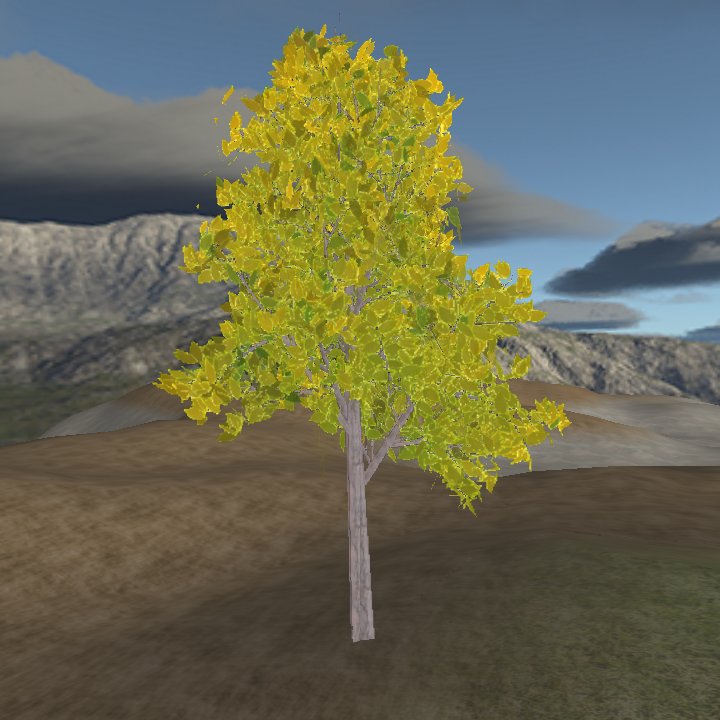
\includegraphics[width=0.17\textwidth]{./testing/LOD1-d10.png}
\\
(a)&(b)&(c)&(d)&(e)
\end{array}$
\end{center}
\caption[Náhledy testovací scény]%
{Náhledy z testování, scéna FRAGMENTS, (a) vzdálenost 50,  (b) vzdálenost 40, (c) vzdálenost 30, (d) vzdálenost 20, (e) vzdálenost 10\label{fig:testFRAG}
}
\end{figure}

grafy

\begin{figure}[here]
\begin{center}
$\begin{array}{cc}
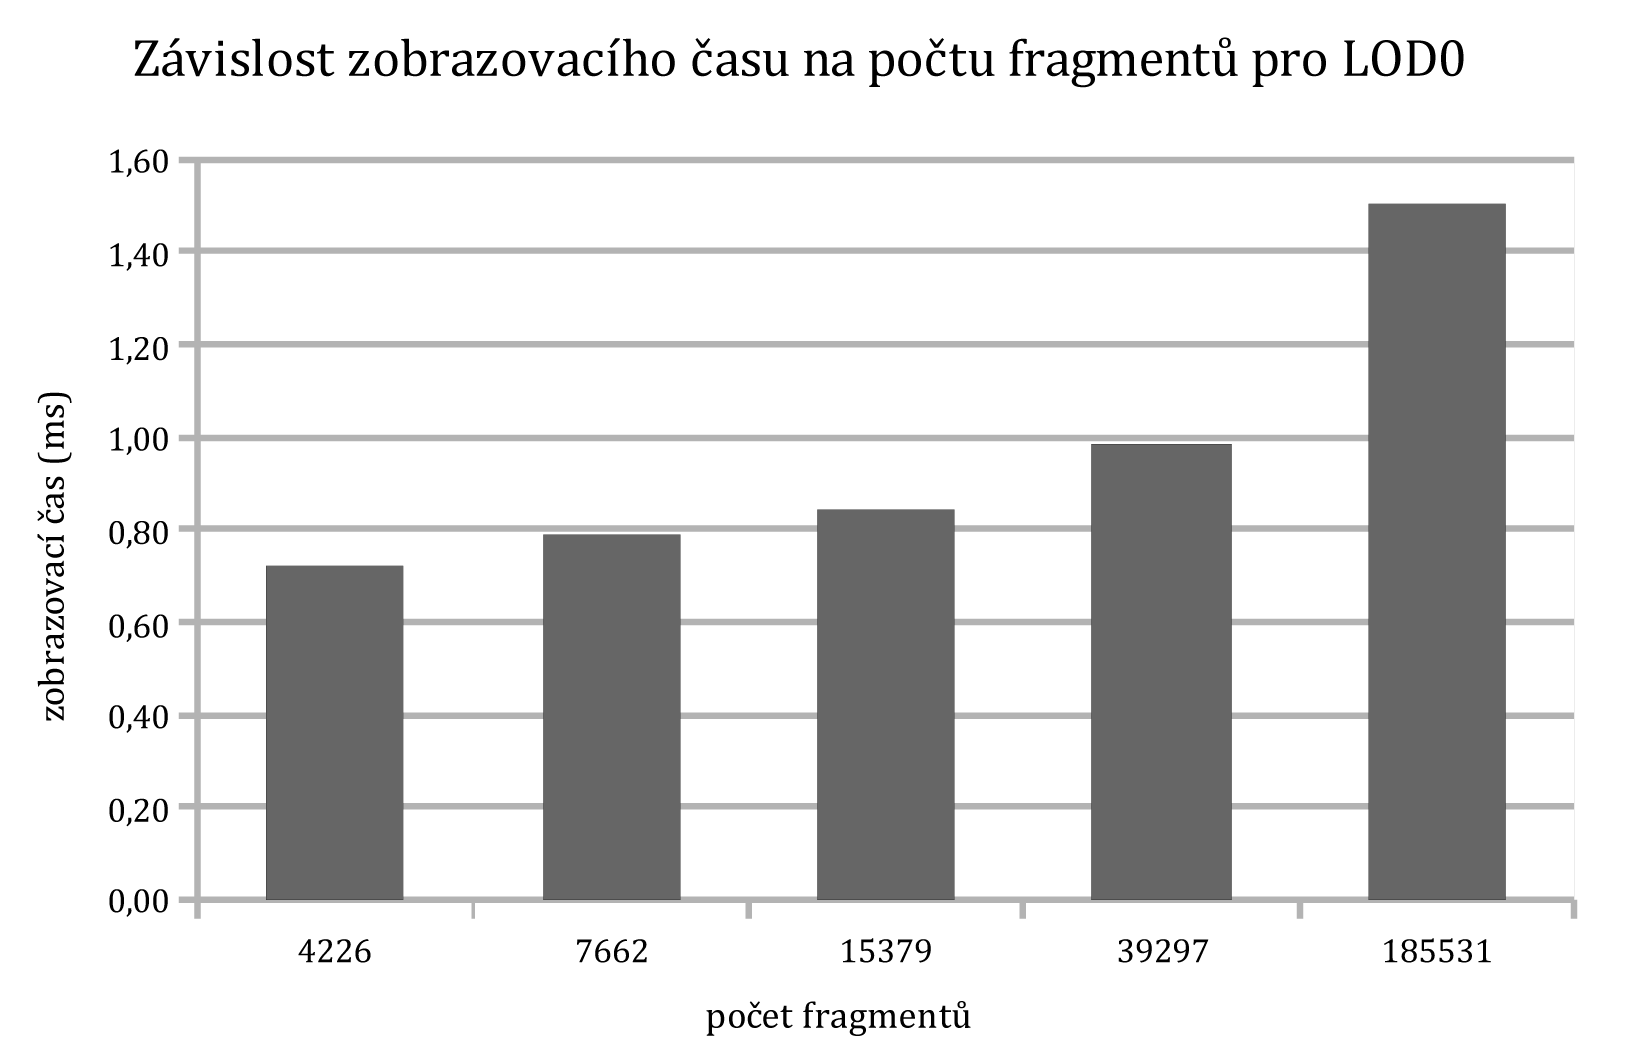
\includegraphics[width=0.5\textwidth]{./graphs/fragLOD0.png}&
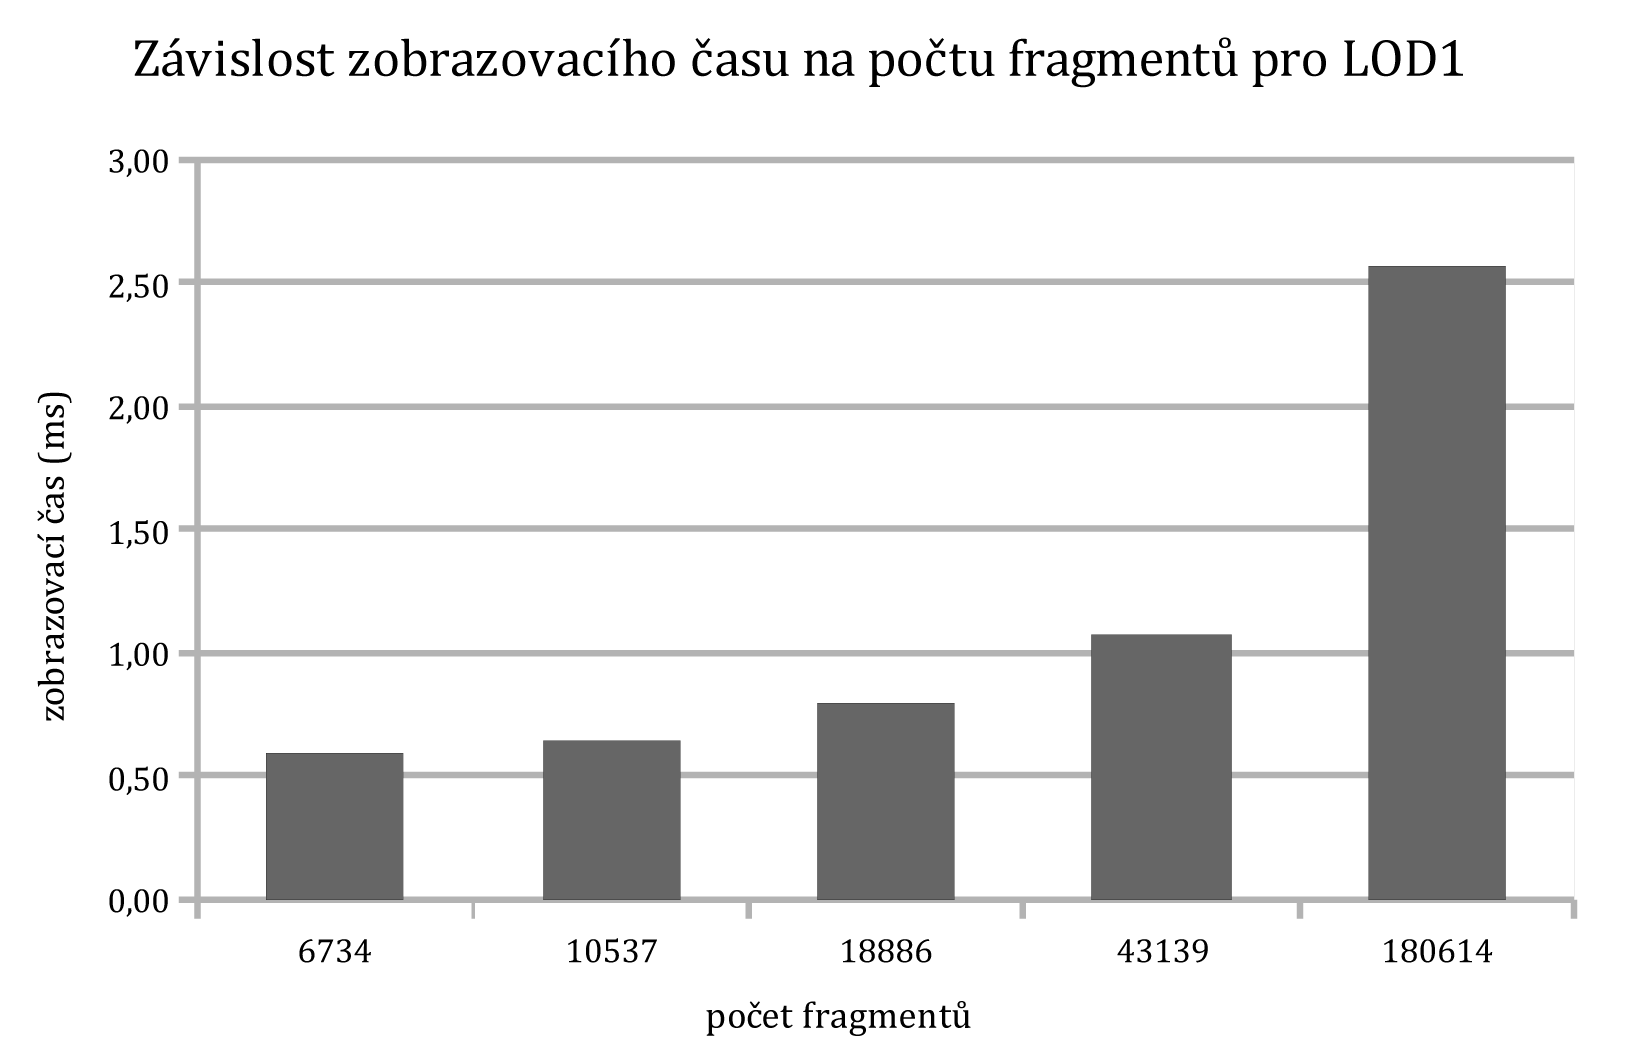
\includegraphics[width=0.5\textwidth]{./graphs/fragLOD1.png}
\\
(a)&(b)
\end{array}$
\end{center}
\caption[Grafy závislosti zobrazovacího času na počtu fragmentů]%
{Grafy závislosti zobrazovacího času na počtu fragmentů\label{fig:testFRAG}
}
\end{figure}



%%%%%%%%%%%%%%%%%%%%%%%%%%%%%%%%%%%%%
%	Podil ruznych LOD na vyslednem case
%
\begin{table}[here]
\centering
\begin{tabular}{|r | c | c | c | c |} 
\hline 
 & fps & čas (ms) & rozdíl časů & \% \\
\hline
bez stromů		&2384,76	&0,42	&0,42	&1,46\\
LOD0			&112,64		&8,88	&8,46	&29,43\\
+LOD1			&36,7		&27,25	&18,37	&63,92\\
+LOD2			&34,79		&28,74	&1,49	&5,19\\
[1ex] 
\hline 
\end{tabular}
\label{table:lod012-contribs}
\caption{Podíly jednotlivých LOD na výsledném čase zobrazení}
\end{table}

\begin{figure}[here]
\begin{center}
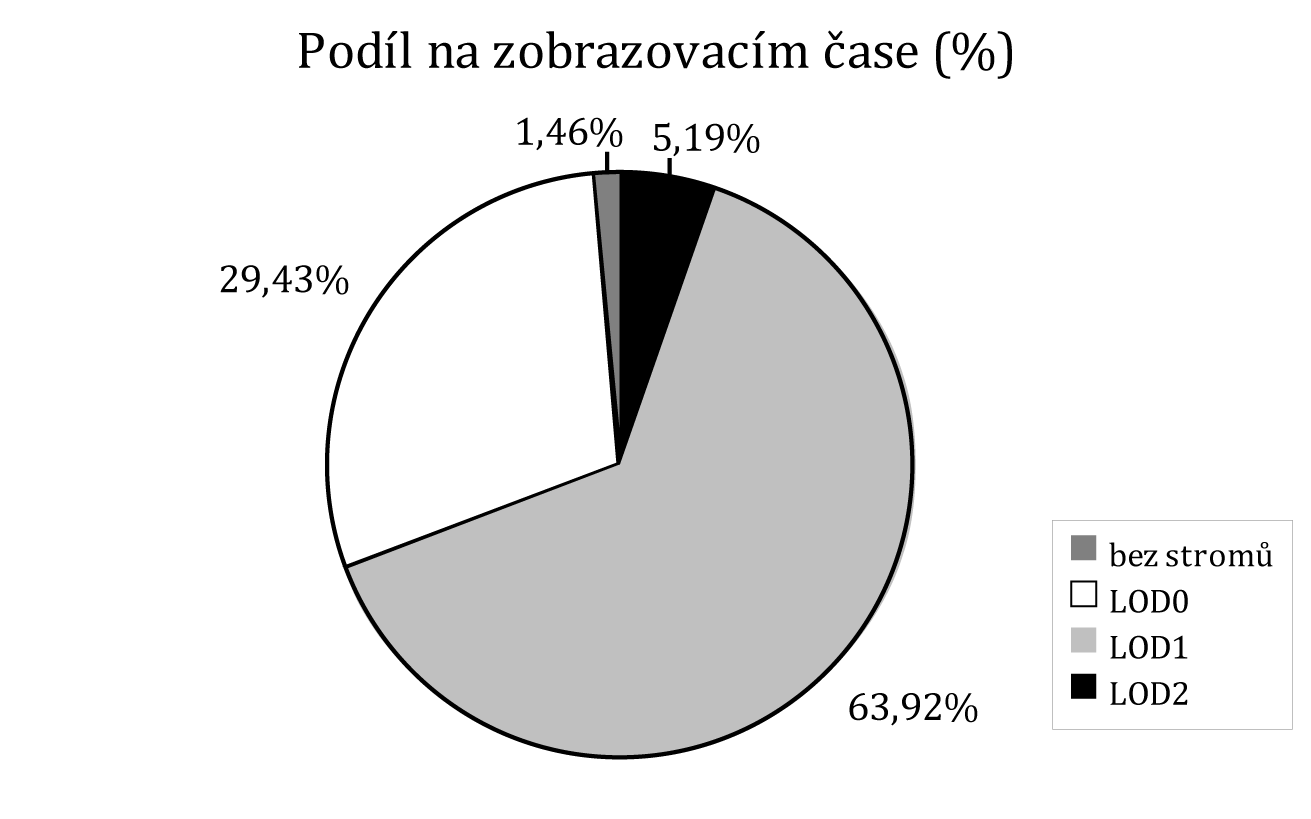
\includegraphics[width=0.6\textwidth]{./graphs/LODsContrib.png}
\end{center}
\caption[Graf podílů jednotlivých LOD na zobrazovacím čase]%
{Graf podílů jednotlivých LOD na zobrazovacím čase\label{fig:testCONTR}
}
\end{figure}

\begin{figure}[here]
\begin{center}
$\begin{array}{ccc}
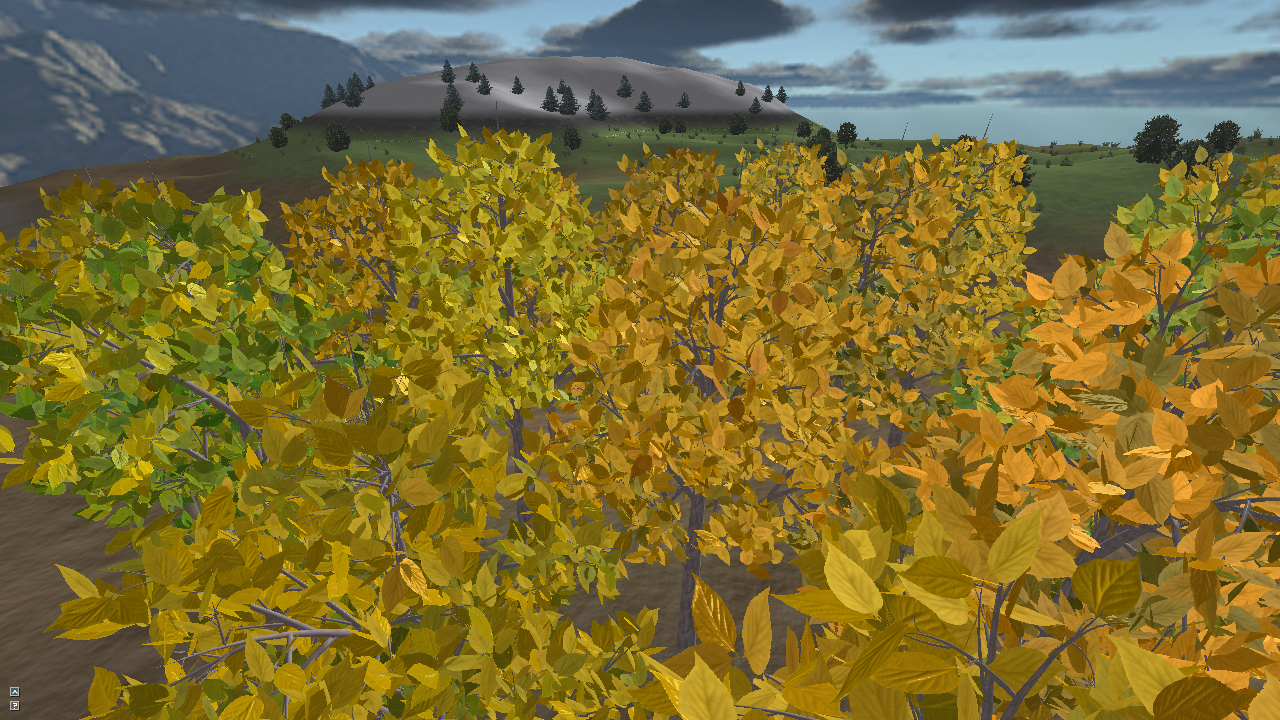
\includegraphics[width=0.31\textwidth]{./testing/on-offLOD0.png}&
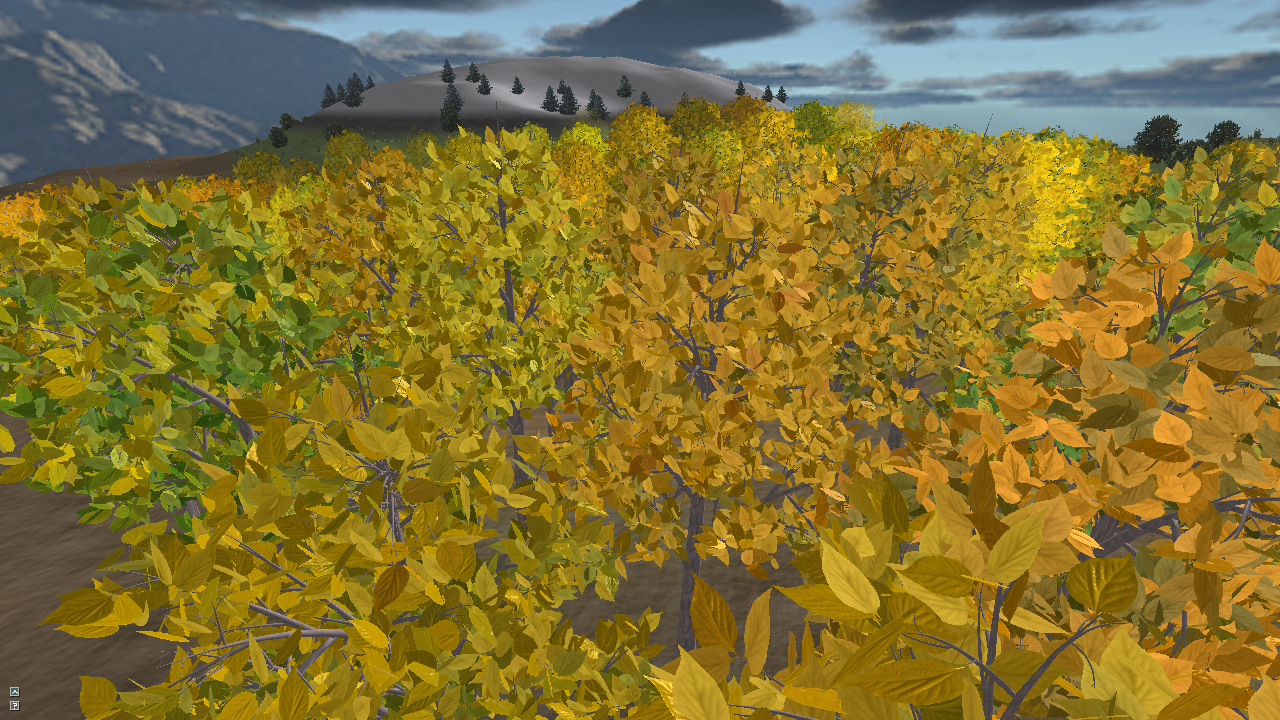
\includegraphics[width=0.31\textwidth]{./testing/on-offLOD1.png}&
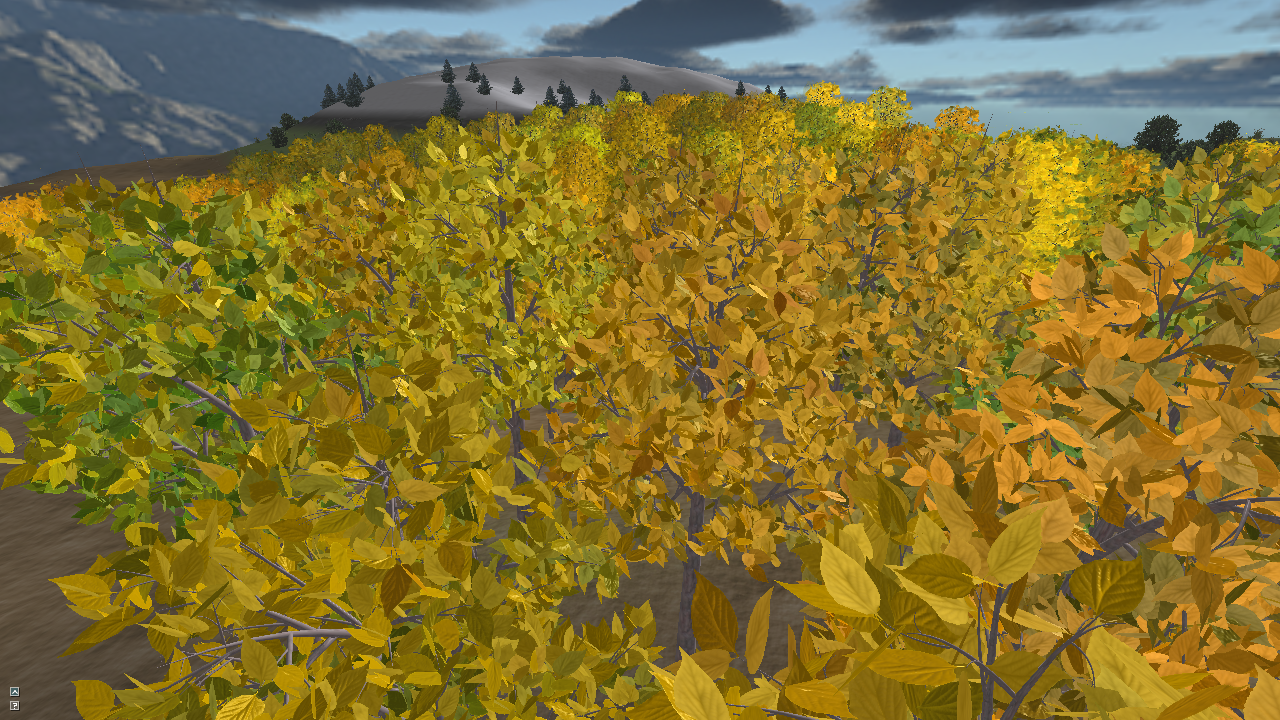
\includegraphics[width=0.31\textwidth]{./testing/on-offLOD2.png}
\\
(a)&(b)&(c)
\end{array}$
\end{center}
\caption[Náhledy testovací scény]%
{Náhledy testovací scény. Zobrazení pouze LOD0 (a), LOD0 a LOD1 (b), všechny LOD (c)\label{fig:testFRAG}
}
\end{figure}

%%%%%%%%%%%%%%%%%%%%%%%%%%%%%%%%%%%%%
%	Ruzne urovne animace
%
\begin{table}[here]
\centering
\begin{tabular}{|r | c | c | c | c || c | c | c | c |} 
\hline 
		&\multicolumn{4}{|c||}{LOD1}		&\multicolumn{4}{c|}{LOD2}\\	
		&\multicolumn{4}{|c||}{\# instancí}	&\multicolumn{4}{c|}{\# instancí}\\
			&10		&25		&50		&100	&10		&25		&50		&100\\
\hline					
bez animace	&1,55	&3,39	&6,35	&11,31	&0,68	&1		&1,73	&2,68 \\
kmen		&2,64	&4,51	&8,14	&13,96	&1,35	&1,74	&3,07	&4,47\\
hlavní větve	&3,84	&7,73	&14,22	&23,53	&1,39	&3,06	&3,83	&4,75\\
listy			&4		&8,45	&16,91	&30,93	&1,79	&3,66	&4,14	&6,44\\
[1ex] 
\hline 
\end{tabular}
\label{table:lod12-anim}
\caption{Vliv podrobnosti animace na zobrazovací čas}
\end{table}

\begin{figure}[here]
\begin{center}
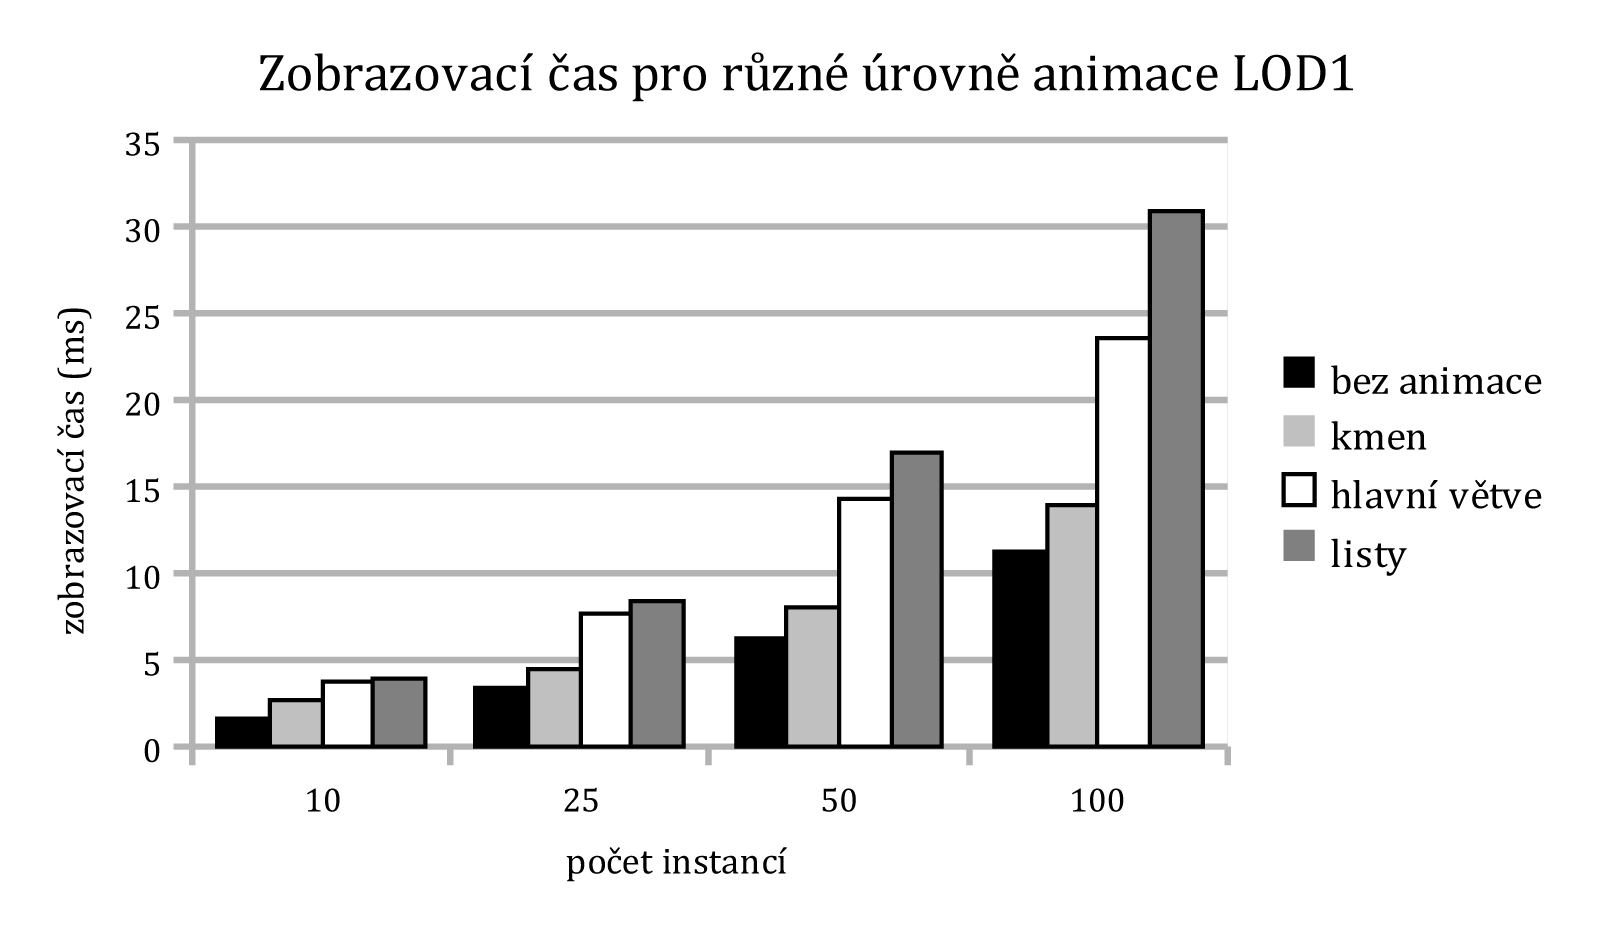
\includegraphics[width=0.75\textwidth]{./graphs/animLOD1.png}
\end{center}
\caption[Graf závislosti zobrazovacího času na podrobnosti animace LOD1]%
{Graf závislosti zobrazovacího času na podrobnosti animace LOD1.\label{fig:testANIM1}
}
\end{figure}
\begin{figure}[here]
\begin{center}
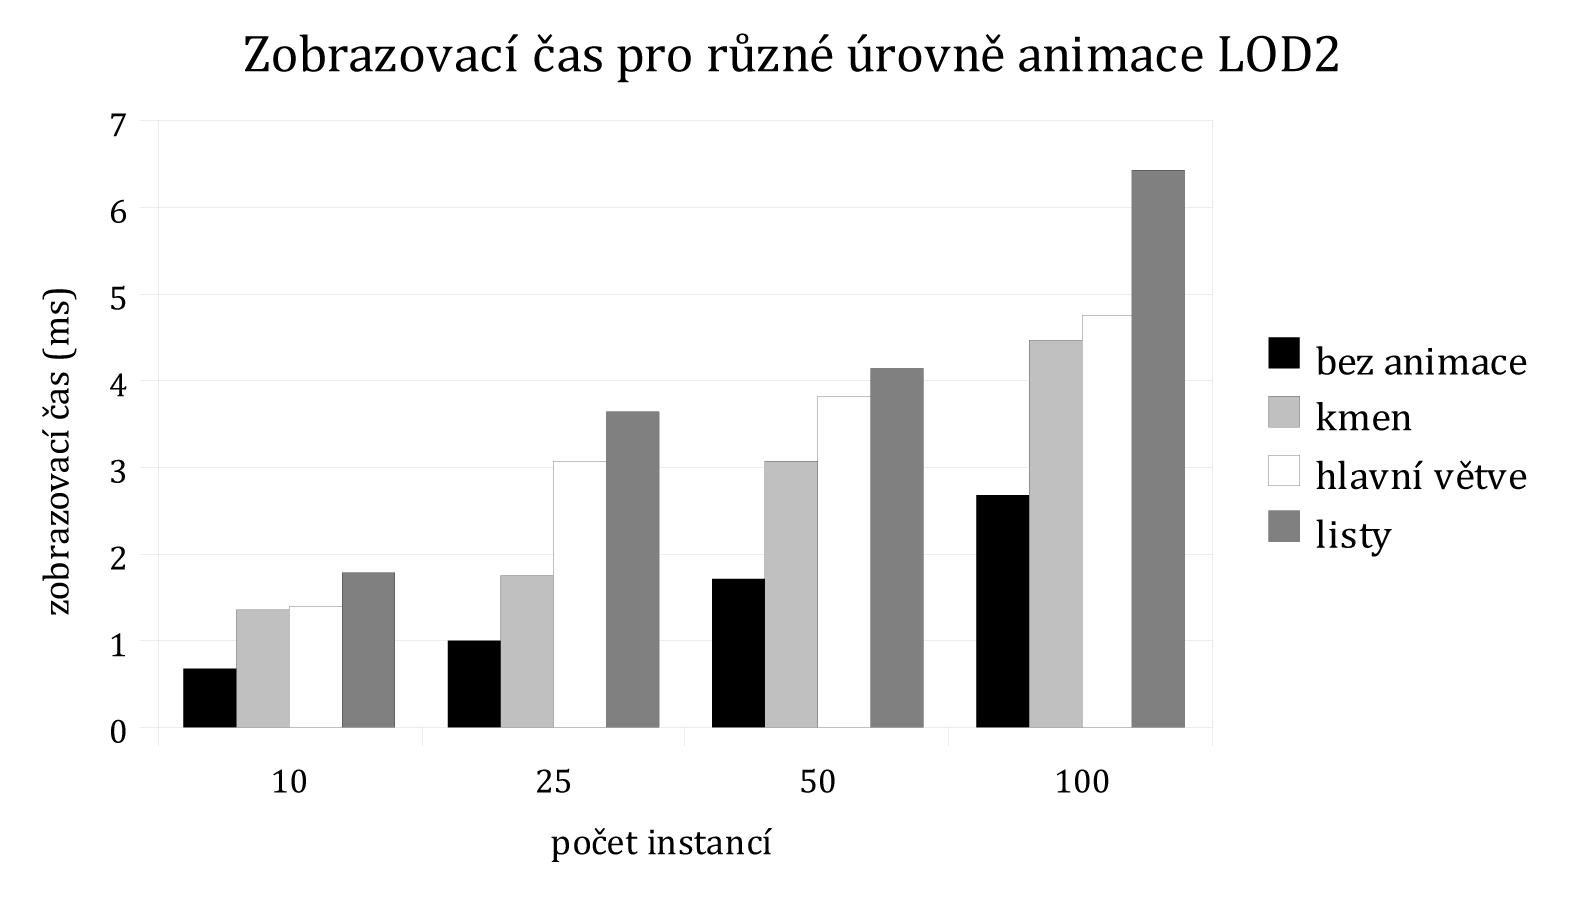
\includegraphics[width=0.75\textwidth]{./graphs/animLOD2.png}
\end{center}
\caption[Graf závislosti zobrazovacího času na podrobnosti animace LOD2]%
{Graf závislosti zobrazovacího času na podrobnosti animace LOD2.\label{fig:testANIM2}
}
\end{figure}


%%%%%%%%%%%%%%%%%%%%%%%%%%%%%%%%%%%%%
%	Shadow mapping
%
\begin{table}[here]
\centering
\begin{tabular}{|r | c | c | c |} 
\hline 
&\multicolumn{3}{|c|}{zobrazovací čas (ms)}\\
rozlišení stínové mapy			&LOD0		&LOD1 (přepis hloubky)	&LOD1 (bez přepisu)\\
\hline					
512 $\times$ 512		&2,26	&3,21	&3,28 \\
1024 $\times$ 1024	&2,44	&3,08	&3,02\\ 
2048 $\times$ 2048	&2,75	&5,98	&5,74\\
[1ex] 
\hline 
\end{tabular}
\label{table:lod01-shadow}
\caption{Vliv rozlišení stínové mapy na zobrazovací čas}
\end{table}